\cleardoublepage

\chapter{Optimización de la eficiencia energética de OmpSs sobre arquitecturas asimétricas}
\label{ch:chapter5}

\section{Descripción de la estrategia de optimización}

\subsection{DVFS sobre la arquitectura big.LITTLE}

\subsection{Evaluación de rendimiento/eficiencia energética de las tareas}


\section{Políticas de reducción de consumo}
\subsection{P1}
Durante la ejecución de un programa paralelo mediante un paradigma basado
en tareas, puede ocurrir el caso en el que en cierto momento de la
ejecución del problema la mayor parte de tareas listas para ser ejecutadas
sean tareas críticas, provocando que nuevas tareas no puedan estar listas
para ejecución hasta que estas tareas críticas finalicen. Este
comportamiento podría reflejarse en una aplicación cuyo grafo de
dependencias se encogiera muy rápidamente en algún punto intermedio de la
ejecución, para luego volverse a expandir rápidamente (un árbol con forma
de diábolo). En este árbol, las tareas del cuello de botella del medio
serían tareas críticas ya que son prioritarias para que la ejecución
continúe su ejecución, y además, en el momento que esto ocurra, un gran
número de tareas estarán listas para ser ejecutadas y
poder continuar la ejecución del problema.\\
Este problema aplicado al planificador botlev (descrito en la
sección~\ref{s3:botlev}) supondría que en el momento en el que el árbol se
estreche, la cola de tareas no críticas tendría un tamaño mucho inferior al
de tareas críticas, y por tanto los cores LITTLE tendrían mucha menor carga
de trabajo que los cores big. Esto ocurriría mientras que los cores big
finalicen la ejecución de sus tareas críticas y se preparen más tareas para
ejecutar por los cores LITTLE.\\
Aunque una forma de intentar paliar este problema sería obligar a que los
cores lentos también ejecutaran tareas críticas, esto podría provocar que
se retrase la finalización de una tarea crítica, ya que aunque su ejecución
aunque puede comenzar antes (pues se disponen de más cores para distribuir
el mismo número de tareas), el rendimiento de los cores LITTLE es mucho
inferior que el de los cores big, provocando retrasos en la ejecución,
incluso llegando a aumentar el problema del cuello de botella.

La política P1 intenta reducir este problema desde un enfoque distinto. La
idea principal que se encuentra detrás de esta política es la de aprovechar
estos momentos en los que la carga de trabajo sobre los cores lentos es
menor para intentar disminuir el consumo energético aplicando una reducción
de frecuencia sobre el cluster LITTLE. Como se podía ver en la
figura~\todo{ref}, reducir la frecuencia al cluster LITTLE implica que la
potencia instantánea consumida disminuye. Es cierto que al reducir la
frecuencia de los cores el tiempo usado en ejecutar una tarea aumenta, pero
como esta técnica únicamente se aplica en los momentos en los que la
ejecución está limitada por el gran número de tareas críticas y el bajo
número de tareas no críticas, se espera que el impacto final en el
rendimiento no sea muy elevado.\\
La forma en la que se ha decidido aplicar esta política sobre botlev
consiste en monitorizar constantemente el número de tareas tanto críticas
como no críticas listas para ser ejecutadas (reflejado en el tamaño de las
colas internas del planificador), y actuar en función a la relación entre
el tamaño de ambas colas. La figura~\ref{s5:fig:listing-p1} muestra un
fragmento esquemático del código encargado de realizar esta tarea. Este
método es invocado cada vez que el tamaño de una cola cambia (ya sea porque
una tarea comienza su ejecución, o porque una tarea se encuentra lista para
ser ejecutada y es insertada en una cola). Como se puede ver en la
línea~\ref{s5:lst:p1-calculoPrincipal(a)}, la frecuencia a la que cambiar
el cluster se calcula como una proporción directa entre el tamaño de ambas
colas, así, si el número de tareas críticas es el doble que el de las
tareas no críticas, la frecuencia se disminuye un ``escalón''; si el tamaño
es el triple, la frecuencia se disminuye hasta el tercer escalón de
frecuencia, etc. Recordar que los valores de frecuencia que puede tomar el
cluster están limitados por el kernel del sistema operativo, como se
mencionó en la sección~\todo{ref}. La
línea~\ref{s5:lst:p1-calculoPrincipal(b)} asegura que la frecuencia final
no es menor que la menor frecuencia soportada. Destacar que con este método
se consigue que el cambio de frecuencia en el cluster se realice de manera
escalonada según varía el tamaño de las colas.\\

\begin{figure}
  \centering

  \begin{lstlisting}[language=C++]
int P1(int bigQueueSize, int littleQueueSize){
  int nxtFreq;
      
  if( littleQueueSize==0 ) nxtFreq = FreqCfg::minLittleFreq; |\label{s5:lst:p1-casoEsp1}|
  else if( bigQueueSize==0 ) nxtFreq = FreqCfg::maxLittleFreq; |\label{s5:lst:p1-casoEsp2}|
  else{
    int idx = min((bigQueueSize / littleQueueSize), |\label{s5:lst:p1-calculoPrincipal(a)}|
                   FreqCfg::maxIdxLittle );         |\label{s5:lst:p1-calculoPrincipal(b)}|
    nxtFreq = FreqCfg::littleFreqs[idx];
  }
  return changeLittleFreq(nxtFreq);
}
\end{lstlisting}

  \caption[Fragmento de código esquemático para la política P1]
  {Fragmento de código esquemático para la política P1.}
  \label{s5:fig:listing-p1}
\end{figure}

Adicionalmente al comportamiento general de esta política, hay que
distinguir dos casos especiales que merecen ser mencionados: el caso en el
que no exista ninguna tarea crítica lista para ser ejecutada, y el caso
opuesto en el que todas las tareas listas sean críticas y los cores lentos
estén totalmente ociosos. En estos casos, las
líneas~\ref{s5:lst:p1-casoEsp1}-\ref{s5:lst:p1-casoEsp2} se encargan de
aumentar la frecuencia al máximo directamente en caso de que todas las
tareas sean no críticas, o de disminuir la frecuencia al mínimo en caso de
que no exista ninguna tarea no crítica que ejecutar.

La figura~\ref{s5:fig:P1-evo} muestra el comportamiento de esta política
para una factoriación de Cholesky de 1024 elementos con precisión simple
dividida en bloques de 64 elementos. La gráfica superior muestra el estado
de las colas durante la ejecución del problema, mientras que la gráfica
inferior muestra la frecuencia del cluster de cores lentos durante toda la
ejecución del problema. Como se puede apreciar, al inicio de la ejecución
donde el número de tareas críticas es elevado, la frecuencia se reduce de
manera escalonada en función de la relación entre el tamaño de ambas
colas. Una vez que el número de tareas no críticas aumenta, el cluster se
mantiene a máxima frecuencia durante la mayor parte de la ejecución hasta
que esta se encuentra en las fases finales donde el número de tareas
críticas vuelve a ser elevado respecto al número de tareas no críticas y la
frecuencia vuelve a disminuirse.

\begin{figure}
  \centering
  \fbox{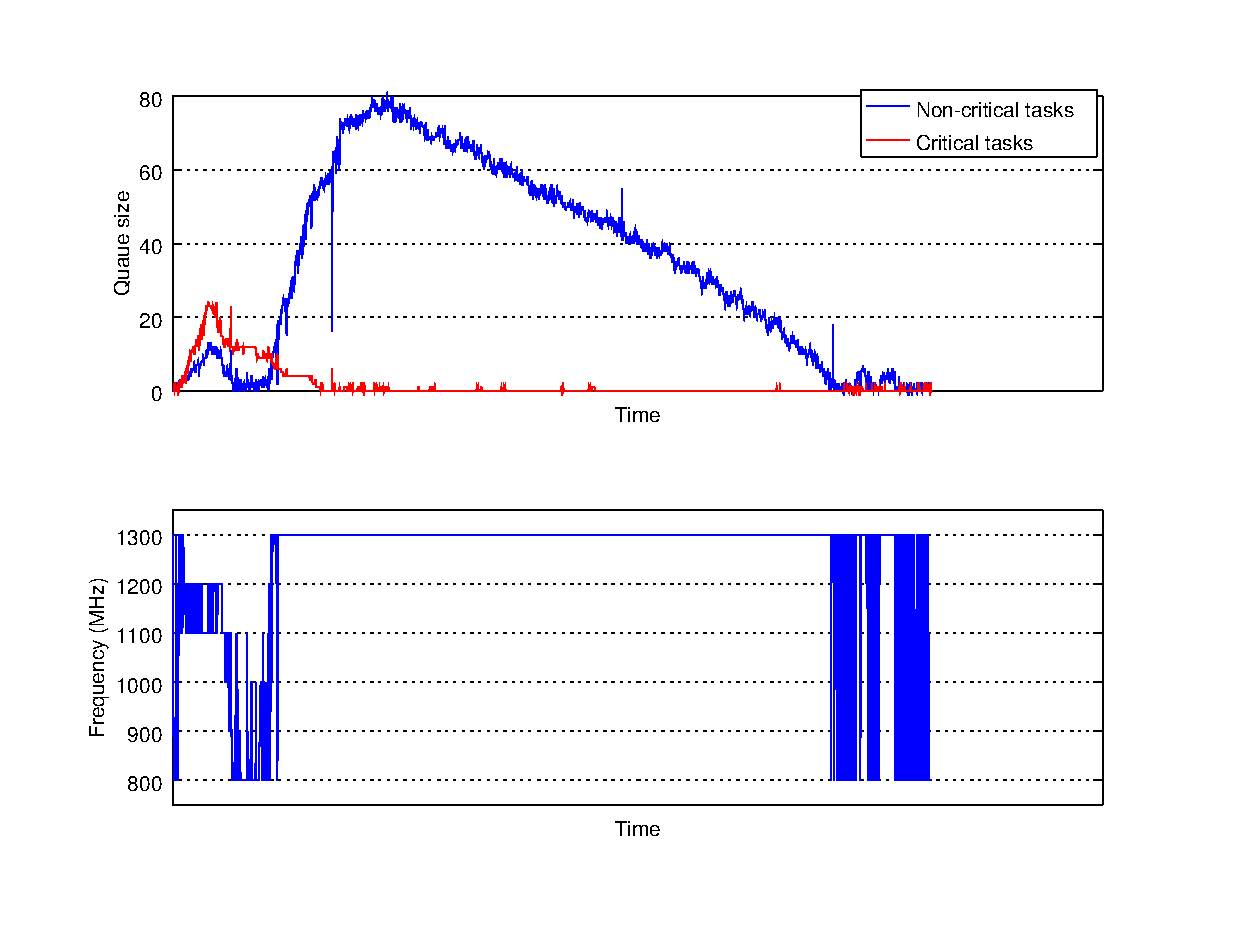
\includegraphics[width=1\textwidth]{Figures/Politicas_evo/P1_1024-64_juno.eps}}
  \caption[Cambio de frecuencias según la política P1]{Cambio de
    frecuencias según la política P1 para una factorización de Cholesky
    sobre una matriz de 1024 elementos dividida en bloques de 64, ejecutada
    sobre la plataforma \juno.}
  \label{s5:fig:P1-evo}
\end{figure}

\subsection{P2 y P2'}
\comentario{Quizás mover esta primera parte a 5.1.1}
A la hora de aplicar técnicas de escalado de frecuencia (DVFS) sobre un
problema cualquiera, la técnica presenta de manera simplificada dos grandes
dimensiones sobre las que tomar decisiones sobre los parámetros de
configuración para conseguir el objetivo de reducir el consumo total:
(a)~una primera dimensión que determina qué frecuencias utilizar durante
los diferentes cambios, y (b)~una segunda dimensión que determina en qué
momentos de la ejecución se debe modificar la frecuencia.\\
La primera dimensión normalmente viene acotada por la propia arquitectura
sobre la que se ejecuta el problema, ya que es común que el procesador no
pueda funcionar a cualquier frecuencia, sino solamente a una serie de
frecuencias prefijadas de antemano. Esto hace que tomar la decisión de a
qué frecuencia se desea configurar el procesador sea únicamente realizar
una elección en un conjunto cerrado y finito de frecuencias. Destacar que
en ocasiones puede ser interesante descartar algunas de estas frecuencias y
no tenerlas en consideración, ya sea porque impactan de manera muy negativa
en el rendimiento, o no tienen un impacto muy significativo en la mejora de
consumo.\\
La segunda dimensión está estrechamente relacionada con el problema a
ejecutar y el conocimiento que se tenga de él. Las decisiones que se pueden
tomar van desde decisiones de grano grueso, como puede ser tener en cuenta
el nivel de carga de trabajo de cada procesador y variar la frecuencia en
función de este dato, hasta decisiones de grano más fino como puede ser
conocer el comportamiento de cada una de las tareas a ejecutar y el árbol
de dependencias de antemano, y tomar decisiones en función de estos
parámetros, por ejemplo, si se sabe que una tarea es crítica, aumentar la
frecuencia para así intentar generar nuevas tareas cuanto antes, o si se
sabe que la ejecución va a estar bloqueada hasta que no finalice una tarea
en concreto, disminuir la frecuencia del resto de procesadores hasta que
esta tarea finalice y así intentar disminuir el consumo energético. Hay que
destacar que aunque bajar la frecuencia del procesador implique conseguir
una potencia instantánea menor, eso no implica que la energía final
consumida sea también menor, ya que al bajar la frecuencia el tiempo de
ejecución puede aumentar lo suficiente para provocar un consumo de energía
mayor global.\\
Adicionalmente a estas dos dimensiones, los sistemas heterogéneos, y en
concreto las arquitecturas asimétricas, presentan una dimensión extra sobre
la que tomar decisiones: (c)~decidir sobre qué elementos de cálculo aplicar
el escalado de frecuencia. En el caso de las arquitecturas asimétricas,
esta decisión se simplifica a decidir si aplicar el escalado al cluster de
cores big, o al cluster de cores LITTLE.\\
\comentario{}

La primera intuición que surge al intentar aplicar un escalado de
frecuencia sobre una arquitectura asimétrica es la de pensar que debido a
la gran diferencia de rendimiento entre los cores big y LITTLE (como se
pudo ver en la figura~\todo{ref}), aplicar una reducción de frecuencia a
los cores big puede suponer una pérdida significativa de rendimiento, lo
cuál puede provocar incluso un aumento en el consumo energético al tardar
mayor tiempo en ejecutarse la aplicación, es decir, se podría llegar a
empeorar tanto el rendimiento como el consumo energético. Para evitar que
suceda este hecho, las políticas P2 y P2' han sido diseñadas para modificar
la frecuencia sobre el cluster de cores LITTLE, y así intentar no causar un
gran impacto sobre el rendimiento. Además, las políticas han sido
desarrolladas sobre el planificador botlev descrito en la
sección~\ref{s3:botlev}, con el objetivo de intentar asegurar que las
tareas críticas se ejecutan en los cores big para así evitar que se
retrasen si se ejecutaran en un core LITTLE con la frecuencia disminuida.\\
Para determinar cuando variar la frecuencia del cluster se tiene en cuenta
el número de tareas listas para ser ejecutadas, así, si existen muchas
tareas para ser ejecutadas, la frecuencia será alta para intentar finalizar
la ejecución cuanto antes, mientras que si existen pocas tareas listas para
ser ejecutadas la frecuencia será menor, intentando favorecer el ahorro
energético. Este planteamiento es similar a tener en cuenta la carga de
trabajo del sistema, pero medida en número de tareas pendientes en vez de
ciclos ociosos/ocupados del procesador. Más concretamente, las políticas
monitorizan el tamaño de la cola de tareas listas para ser ejecutadas, y
determinan cuál es el tamaño máximo de la cola hasta el momento de manera
dinámica. Si la cola posee un tamaño igual o superior al tamaño máximo
conocido, significa que el número de tareas es elevado y por tanto la
frecuencia debe ser elevada. Si el tamaño es menor, entonces se determina
en que porcentaje es menor, y en función de las frecuencias consideradas se
toma la decisión de modificar la frecuencia actual o no. En el código de la
figura~\ref{s5:fig:listing-p2} se muestra el pseudocódigo asociado a estas
políticas. El bloque \texttt{if} de la línea~\ref{s5:lst:p2-detectPico} es
el encargado de determinar si el tamaño actual de la cola es mayor o igual
que cualquier tamaño hasta el momento, y en caso de ser así, configurar el
cluster para que funcione a máxima frecuencia. Esto es equivalente a
determinar si hay un pico de carga de trabajo o no. Las
líneas~\ref{s5:lst:p2-tamStep1}-\ref{s5:lst:p2-tamStep2} determinan el
número de tareas que separan una frecuencia de la otra. La forma de
determinar esta cantidad consiste en repartir de manera equitativa el
espacio máximo de tareas conocido hasta el momento entre todas las
frecuencias, y asignar la frecuencia actual en función de qué tamaño posea
la cola (línea~\ref{s5:lst:p2-step}). Por ejemplo, si el cluster es capaz
de ejecutarse a 5 frecuencias distintas, y hasta el momento el número
máximo de tareas preparadas para ser ejecutas ha sido de 20 tareas, antes
de cambiar de frecuencia se dispone de un margen de 4 tareas. Si el tamaño
actual de la cola es de 3 tareas, la frecuencia del cluster será la mínima,
mientras que si es de 5 tareas, la frecuencia ya no será la mínima, sino la
frecuencia inmeditamente superior.

\begin{figure}
  \centering

  \begin{lstlisting}[language=C++]
int P2(int littleQueueSize, int bigQueueSize){      
  //Comprobamos si estamos en un pico de carga
  if(littleQueueSize >= FreqCfg::maxQueueSize){ |\label{s5:lst:p2-detectPico}|
    FreqCfg::maxQueueSize = littleQueueSize;

    return changeLittleFreq(FreqCfg::maxLittleFreq);
  }

  //Tamanyo para cambiar de frecuencia
  float tamStep = (FreqCfg::maxQueueSize*1.0 /     |\label{s5:lst:p2-tamStep1}|
                   (FreqCfg::maxIdxLittle+1)*1.0); |\label{s5:lst:p2-tamStep2}|
  //Escalon actual
  int step = (int) (littleQueueSize / tamStep);    |\label{s5:lst:p2-step}|

  return changeLittleFreq(FreqCfg::littleFreqs[step]);
}
  \end{lstlisting}

  \caption{Pseudocódigo para las políticas P2 y P2'.}

  \label{s5:fig:listing-p2}
\end{figure}

La diferencia entre las políticas P2 y P2' se encuentra en el rango de
frecuencias que se consideran para el cluster. Así, la política P2 divide
el tamaño de la cola entre todas las frecuencias posibles para el
procesador, mientras que la política P2' solamente considera la frecuencia
máxima y mínima del mismo. 


\subsection{P3}
La política P3 es similar a la política anterior P2, pero realizando el
escalado de frecuencias sobre el cluster de cores big en vez de cores
LITTLE. De manera similar a la anterior, la política ha sido implementada
sobre el planificador botlev implementado sobre \ompss para intentar
minimizar el impacto negativo sobre las tareas críticas. La
figura~\ref{s5:fig:P3-evo} muestra los distintos cambios de frecuencia que
se han realizado en función del número de tareas listas para ser
ejecutadas. En la parte superior, se muestra la evolución del número de
tareas listas para ser ejecutadas según avanza la ejecución del
problema. En la gráfica inferior, se muestra la frecuencia del cluster de
cores big durante la ejecución. Ambas gráficas poseen la misma escala en el
eje x, permitiendo relacionar ambas gráficas de manera visual. La gráfica
corresponde a una ejecución sobre la plataforma Juno, para una
factorización de Cholesky sobre una matriz de tamaño 4608 elementos
dividida en bloques de tamaño 512 elementos en precisión simple.\\


\begin{figure}
  \centering
  {
    \setlength{\fboxsep}{-10pt}
    \fbox{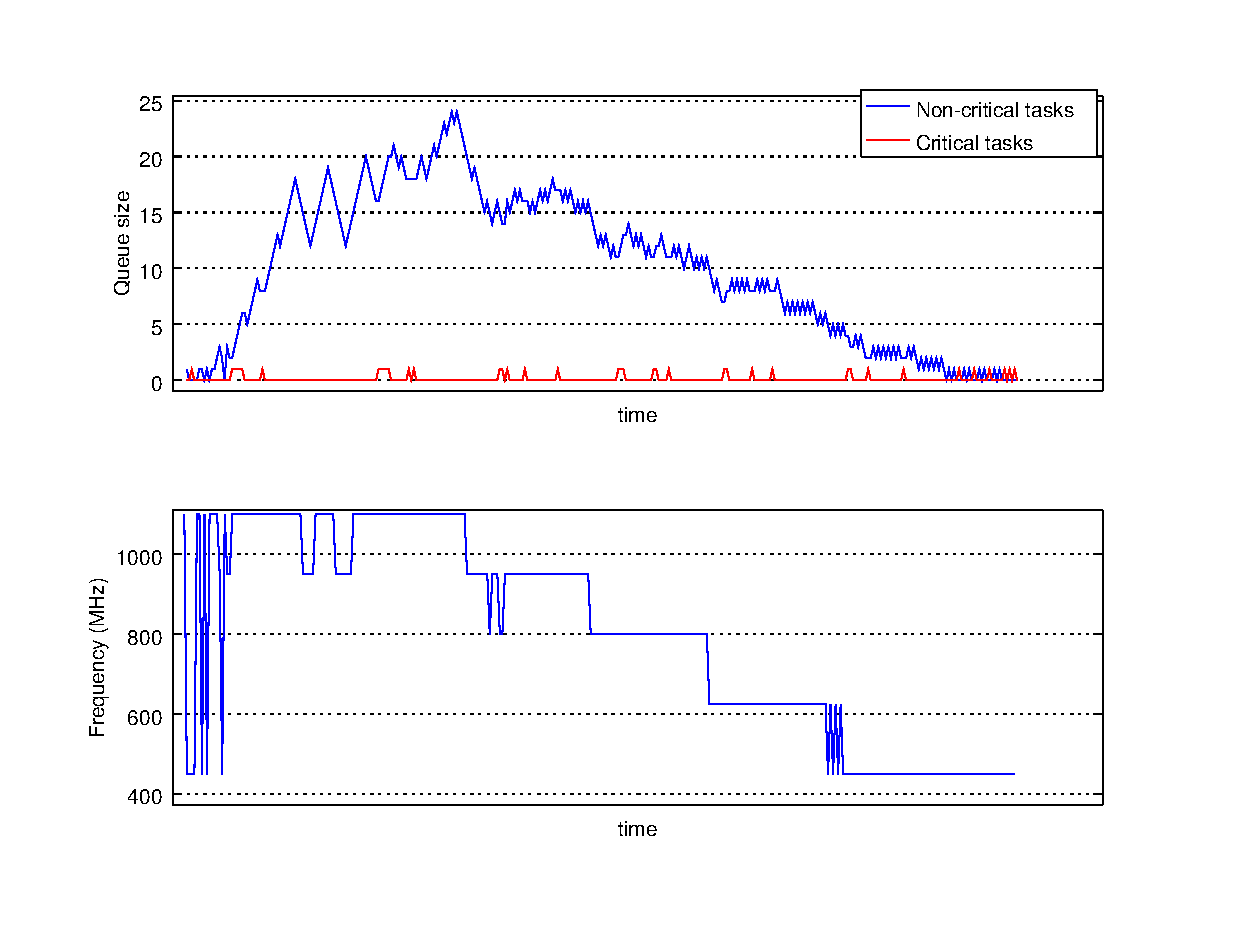
\includegraphics[width=1.0\textwidth]{Figures/Politicas_evo/P3_4608-512.eps}}
  }
  \caption[Escalado de frecuencia en función del número de tareas listas
  según la política P3]{Escalado de frecuencia en función del número de
    tareas listas según la política P3. La ejecución corresponde a una
    factorización de Cholesky sobre una matriz de 4608 elementos en
    precisión simple, dividida en bloques de tamaño de 512 elementos,
    ejecutada sobre la plataforma de desarrollo Juno (donde los cores big
    corresponden a cores ARM-A57).}
  \label{s5:fig:P3-evo}
\end{figure}


Como se puede observar en la gráfica, la ejecución se puede dividir en dos
partes diferenciadas: una primera parte hasta que alcanza la cola el tamaño
máximo, y una segunda parte en la que el número de tareas críticas
desciende constantemente. Estas dos partes están totalmente relacionadas
con el grafo de dependencias de una factorización de Cholesky, donde existe
una primera fase en la que se crean un gran número de tareas y se expande
el árbol, y una segunda fase donde las tareas se van ejecutando y el árbol
se cierra poco a poco.\\
Como el cálculo del tamaño máximo de la cola se realiza de manera dinámica,
en la primera fase se realizan cambios de frecuencia continuamente, a cause
de ligeros cambios en el tamaño de la cola hasta que se consigue
estabilizar la cota superior, y poder aplicar la política de manera
correcta. Una vez que se alcanza el tamaño máximo de la cola, se observa
como el espacio está dividido en varios escalones, cada uno correspondiente
a una frecuencia distinta. En algunos puntos en los que el tamaño de la
cola crece en alguna unidad, se observa que la frecuencia oscila hasta que
se vuelve a estabilizar el decrecimiento del número de tareas. Esto se
observa fácilmente al comienzo de la fase en la que el procesador se
encuentra a una frecuencia de 950 MHz, como la caída del número de tareas
es elevada y en algunos puntos la frecuencia se disminuye a 800MHz. También
se puede observar en la fase final de la ejecución, donde la frecuencia
varía entre 450MHz y 625MHz.


\subsection{P4 y P5}
Las políticas descritas hasta el momento intentan obtener una mejora en el
consumo energético a partir de un escalado de frecuencia en los distintos
clusters de la arquitectura, prestando atención al número de tareas listas
para ser ejecutadas como medida equivalente a detectar el nivel de carga de
trabajo en un cierto momento. Estas políticas se han desarrollado prestando
atención a la figura~\todo{ref}, en la que se puede observar la disminución
del consumo energético en función de la frecuencia. La siguiente idea que
surge prestando atención a la figura es la de intentar disminuir el consumo
al no utilizar algún cluster durante parte de la ejecución. Como se puede
observar el consumo energético es menor si el cluster no se usa,
independientemente de la frecuencia utilizada. Las siguientes políticas han
sido diseñadas con el objetivo de que en ciertos momentos de la ejecución,
modificar el planificador de tareas para evitar que se asignen tareas a
cierto cluster del sistema. Es decir, estas políticas no están orientadas a
realizar técnicas de escalado de frecuencia, sino que tratan con el
problema de planificación de tareas a los distintos \wts disponibles.\\

La política P4 monitoriza el tamaño de las colas de tareas listas y en
función del tamaño de la cola respecto al tamaño máximo (similar a la
política P2 o P3), decide si asignar tareas listas al cluster de cores
LITTLE o no. En caso de que el tamaño de la cola sea lo suficientemente
pequeño, la política no asigna ninguna tarea lista al cluster, provocando
que este se encuentre ocioso. Hay que mencionar que aunque el planificador
no asigne tareas al cluster, esto no implica que el sistema operativo no
ejecute procesos sobre él, pero el impacto final es mínimo comparado con el
de ejecutar una tarea o no.\\
Para realizar este proceso, cada vez que una tarea se inserta en la cola de
tareas listas o es extraída de esta, se compara el tamaño actual de la cola
con el tamaño máximo conocido hasta el momento, y se decide si se debe
utilizar el cluster o no para ejecutar acciones. Una vez que un \wt
finaliza la ejecución de una tarea, éste solicita una nueva tarea a
ejecutar al planificador. Si el \wt se ejecuta sobre un core del cluster
LITTLE, y se ha decidido que el cluster no ejecute ninguna acción, al \wt
se le asigna una tarea nula, evitando así la ejecución de cualquier tarea
en ese core asociado al \wt y perteneciente al cluster inhabilitado. En
caso de que el cluster no se encuentre desactivado se asigna la siguiente
tarea de la cola de tareas listas para que la ejecute el \wt.\\
Para que esta política funcione, es necesario que se verifiquen algunas
condiciones cuando se ejecute el problema:

\begin{itemize}
\item Para simplificar la tarea, el número de \wts lanzados debe coincidir
  con el número de núcleos de la placa. En caso de que el número de \wts sea
  superior, ocurriría que varios \wts estarían compitiendo por ejecutarse
  simultáneamente en el mismo núcleo. De manera contraria, si el número de
  \wts es menor que el número de núcleos, se estarían desaprovechando
  recursos ya que no se utilizarían todos los cores de manera simultánea. En
  \nanos esto se consigue mediante el argumento \texttt{--smp-workers=<n>}.
\item Cada \wt debe estar asignado a un núcleo único de la placa,
  provocando que un \wt siempre ejecute tareas en el mismo núcleo durante
  todo el problema. Esta condición unida a la anterior implica que existe una
  relación directa entre cada núcleo y cada \wt del \emph{runtime}. En
  \nanos, este comportamiento se consigue desactivando la opción contraria
  mediante el argumento \texttt{--disable-binding}.
\item Aunque se tenga control sobre qué tarea se ejecuta en qué \wt (y por
  tanto en qué core), existen ciertas tareas pertenecientes al propio
  \emph{runtime} o código no paralelo del programa sobre el que no se puede
  tomar decisiones desde el planificador, siendo normal que este código se
  ejecute sobre el \wt principal, normalmente ejecutado sobre el núcleo 0 de
  la máquina.
\end{itemize}


En las políticas anteriores donde se disponía un número limitado de
frecuencias, el punto en el que cambiar la frecuencia venía determinado a
la hora de repartir por igual el tamaño máximo de la cola entre todas las
frecuencias disponibles. Para dar mayor flexibilidad a esta política, el
punto en el que tomar la decisión de apagar el cluster viene determinado
por una variable de entorno elegida por el usuario a la hora de lanzar el
experimento. Esto permite observar el comportamiento variando el momento en
el que se desactiva el cluster, como se describe en la siguiente
sección. Además, para evitar efectos rebote, en los que el clustes esté
activando y desactivándose de manera continuada, mediante experimentación
se ha decidido insertar un margen del 10\% del tamaño de la cola antes de
tomar la decisión de apagar o encender el cluster.\\

La figura~\ref{fig:P4-puedo-ejecutar} muestra un fragmento del código
encargado de determinar si un \wt debe ejecutar una tarea lista o no. La
función recibe por parámetro el núcleo al que se encuentra asignado el \wt
y devuelve un valor \emph{booleano} en función de si el cluster se
encuentra desactivado o no. Para agilizar el proceso, la
línea~\ref{lst:p4-a} filtra la ejecución y permite continuar con la
ejecución únicamente en el caso de que el cluster se encuentre
desactivado. La labor de determinar si el cluster debe estar activo o no se
realiza en el momento en el que una tarea lista es insertada en la cola de
tareas listas, o es extraída, y se realiza mediante un código muy parecido
al de la figura~\ref{s5:fig:listing-p2}.\comentario{quizá poner el código
  real}. Si el cluster se encuentra desactivado, mediante las siguientes
líneas se determina si el núcleo pertenece al cluster desactivado. En caso
de pertenecer, se devuelve el valor de falso para indicar que el \wt no
debe ejecutar nada, pero además se reduce la frecuencia de núcleo al mínimo
para intentar minimizar el consumo energético mientras no se utilice el
cluster de cores LITTLE (línea~\ref{lst:p4-c}).


\begin{figure}
  \centering
\begin{lstlisting}[language=C++]
bool CoresCfg::puedoEjecutar(int coreId){
  //core little
  if(apagadoLittle)                     |\label{lst:p4-a}|
    for(int i=0; i<N_CORE_LITTLE; i++)
      if(coresLittle[i] == coreId){     |\label{lst:p4-b}|
        if (!coresApagados[coreId]){
          FreqCfg::changeLittleFreq(FreqCfg::minFreqLittle); |\label{lst:p4-c}|
          coresApagados[coreId] = true;   |\label{lst:p4-d}|
        }
        return false;
      }
\end{lstlisting}
  \caption{Fragmento de código para determinar si asignar una tarea a un
    \wt o no.}
  \label{fig:P4-puedo-ejecutar}
\end{figure}

La política P5 realiza el mismo procedimiento, pero para el cluster de
cores big. Ambas políticas están implementadas sobre el planificador botlev
para así asegurar que la ejecución de tareas críticas siguen siendo en
cores big. Sin embargo, al apagar los cores big, hay que tener en cuenta
que es necesario que las tareas críticas se ejecuten en cores LITTLE si los
big no están disponibles para que la ejecución no se quede bloqueada por
las tareas críticas (opción \texttt{--steal=1} en botlev).\\
La figura~\ref{fig:P4-evo} muestra un ejemplo de esta política para la
ejecución de una factorización de Cholesky. La gráfica superior muestra la
ejecución de las diferentes tareas por los distintos \wts, cada uno
asignado a un núcleo distinto en orden de aparición. La ejecución ha sido
realizada sobre la plataforma \juno, por lo que los 4 primeros núcleos
corresponden a cores LITTLE, mientras que los dos siguientes a cores
big. La segunda gráfica muestra la evolución del tamaño de las colas en
función del tiempo. Como se puede observar, la ejecución de las tareas se
realiza de manera normal hasta que el tamaño de la cola decrece por debajo
del 25\% del tamaño máximo (el experimento se configuró con este valor). En
ese momento, los cores LITTLE dejan de recibir tareas mientras que los big
continúan su ejecución normal. Una vez que el número de tareas vuelve a
incrementarse, los cores lentos vuelven a activarse y a ejecutar tareas,
hasta que al final de la ejecución el tamaño de la cola vuelve a decrecer,
y el cluster se desactiva hasta finalizar la ejecución. Aunque el primer
\wt está asociado a un core LITTLE, también es considerado como el \wt
principal del planificador, por lo que es el encargado de ejecutar la parte
del código no paralela (en color verde). La mayor parte del tiempo que se
encuentra ejecutando este código corresponde a tareas del propio
planificador, o a la espera de que finalice la ejecución paralela (marcada
por una etiqueta \texttt{\#pragma omp taskwait} en el código secuencial),
por lo que el impacto final no es muy significativo.



\begin{figure}
  \centering
  \begin{framed}
    \begin{subfigure}{1\textwidth}
      \centering
      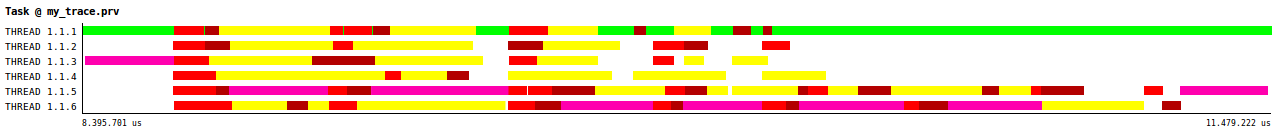
\includegraphics[width=1\linewidth]{Figures/Politicas_evo/Apagado_tareas.png}
      \caption{Asignación tareas a los distintos \wts.}
      \label{}
    \end{subfigure}

\vspace{0.5cm}

    \begin{subfigure}{1\textwidth}
      \centering
      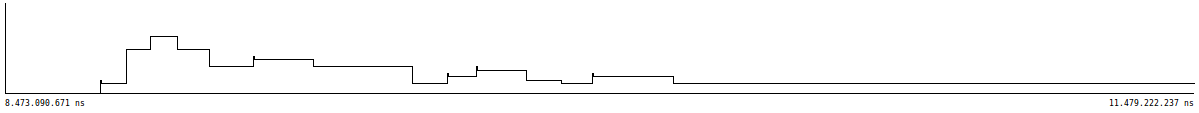
\includegraphics[width=1\linewidth]{Figures/Politicas_evo/Apagado_colas.png}
      \caption{Evolución del tamaño de la cola de tareas listas.}
      \label{}
    \end{subfigure}  
    
    % \begin{subfigure}{0.9\textwidth}
    %   \centering
    %   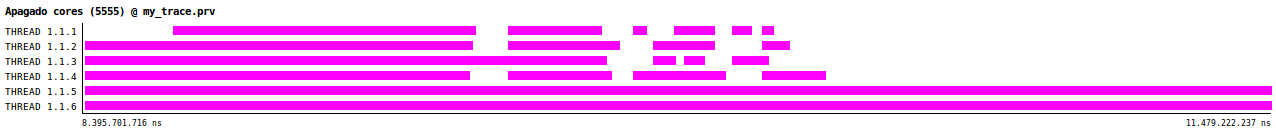
\includegraphics[width=1\linewidth]{Figures/Politicas_evo/Apagado_cores.png}
    %   \caption{Estado de los núcleos. Rosa = activo. Blanco = inactivo.}
    %   \label{}
    % \end{subfigure}  
  \end{framed}
  \caption[Asignación de tareas en función del tamaño de la cola según la
  política P4]{Asignación de tareas en función del tamaño de la cola según
    la política P4. La gráfica superior muestras las distintas tareas
    ejecutadas por cada uno de los \wts a lo largo del tiempo. Clave de
    colores: rojo=\trsm, rosa=\potrf, granate=\syrk, amarillo=\gemm,
    verde={\sc main}. La ejecución corresponde a una factorización de
    Cholesky para una matriz de 4096 elementos dividido en bloques de
    tamaño 512 en precisión simple sobre una arquitectura \juno, donde los
    4 primeros \wts corresponden a los cores lentos y los 2 últimos a los
    cores rápidos. La política está configurada para desactivar cores a
    partir del 25\% del tamaño máximo de la cola.}
  \label{fig:P4-evo}
\end{figure}



\subsection{P6}
Una de las muchas funcionalidades que ofrece el kernel Linux es la de poder
activar y desactivar cores a demanda y de manera dinámica. En cualquier
momento de la ejecución, un núcleo puede ser desactivado, y este desaparece
del sistema, siendo totalmente transparente para cualquier aplicación en
ejecución. Esto implica que si se decide apagar un core, todos los procesos
asociados a ese núcleo son migrados a otro de manera totalmente
transparente al proceso en ejecución, el número total de cores disminuye y
cualquier llamada a una función del kernel considerará la nueva
configuración hardware creada como la configuración real de la
máquina. Esta funcionalidad permite, entre muchas cosas, la de generar
arquitecturas diferentes utilizando el mismo hardware.

Esta funcionalidad aplicada a una arquitectura big.LITTLE teóricamente
proporciona que en cualquier momento de la ejecución se pueda desactivar
uno de los dos cluster de la máquina, convirtiendo a la arquitectura en una
plataforma totalmente simétrica. En la práctica, no todas las versiones
del kernel permiten apagar el core 0, por lo que no es posible apagar el
cluster entero que contiene a este core.

Para realizar un estudio del impacto que tiene apagar cores sobre el
consumo energético, se ha realizado el experimento de desactivar uno a uno
mientras se mide el consumo de ambos clusters. Además, para evitar
errores en las medidas, se ha establecido un tiempo de espera entre apagado
de dos cores, y adicionalmente se ha ejecutado el test asociado a un core
que no se fuera a apagar, evitando así problemas al migrar el proceso de un
core a otro. La figura~\ref{s5:fig:apagadoCores} muestra las mediciones del
consumo energético en las dos plataformas: la figura superior para la
plataforma \juno y la inferior para la plataforma \odroid.

\comentario{Bajar el numero de puntos. Tarda mucho en renderizar}
\begin{figure}
  \centering
  \begin{subfigure}{0.9\textwidth}
    \centering
    \fbox{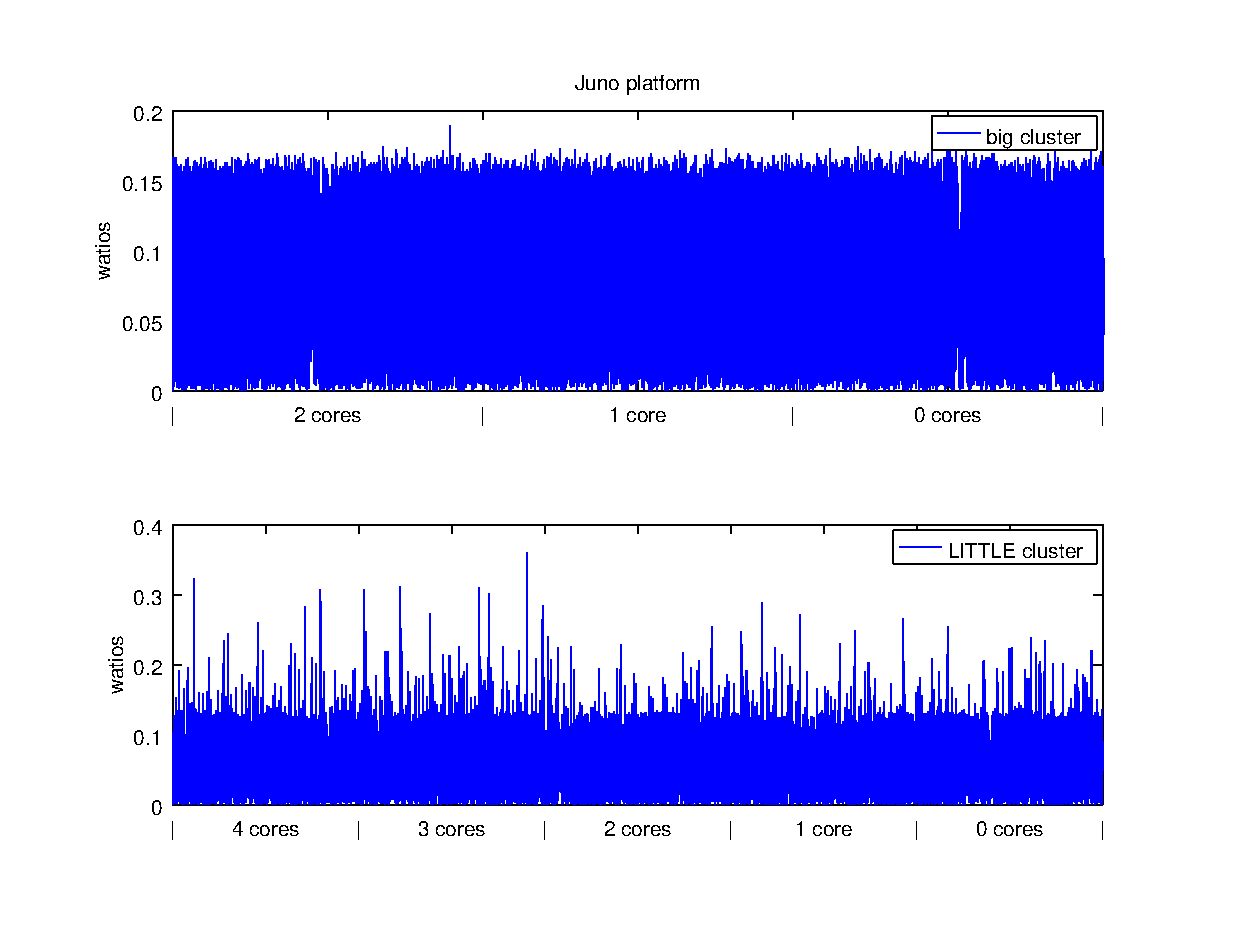
\includegraphics[width=0.75\linewidth]{Plots/Modelos_consumo/apagadoJuno.eps}}
    \caption{Plataforma \juno: 2 cores big A57 y 4 cores LITTLE A53.}
      \label{}
    \end{subfigure}
\vspace{0.5cm}

    \begin{subfigure}{0.9\textwidth}
      \centering
      \setlength{\fboxsep}{20pt} %No tienen el mismo margen :(
      \fbox{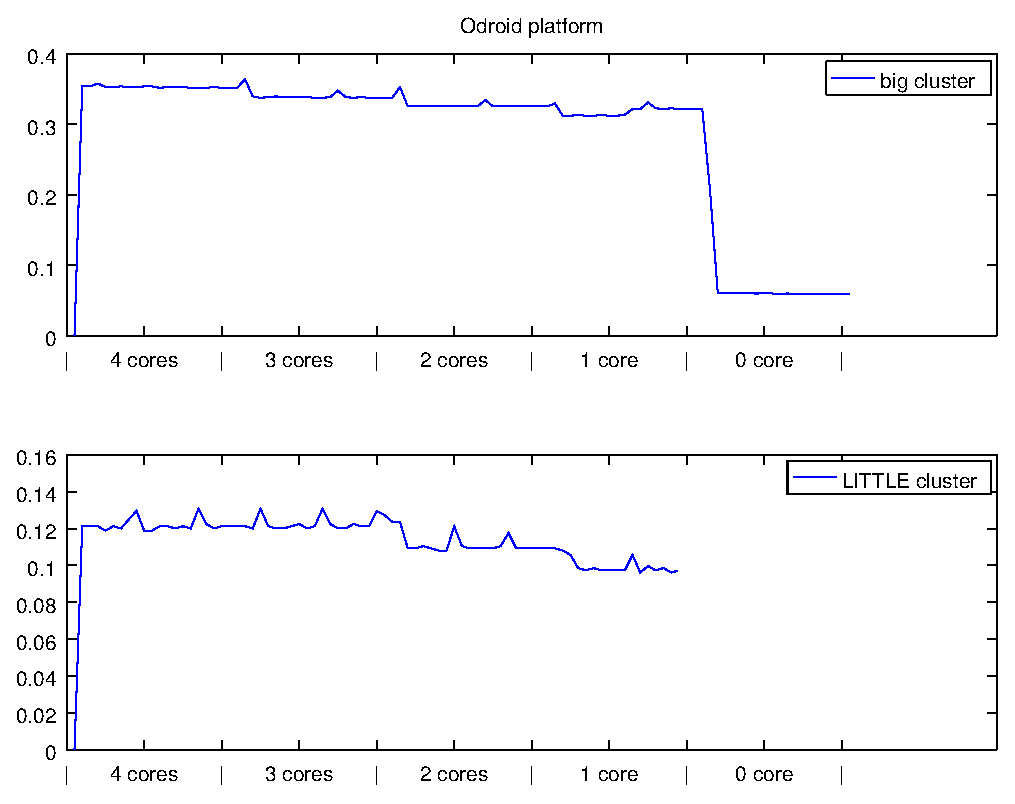
\includegraphics[width=0.66\linewidth]{Plots/Modelos_consumo/apagadoOdroid.eps}}
      \caption{Plataforma \odroid: 4 cores big A15 y 4 cores LITTLE A7.}
      \label{}
    \end{subfigure}  
    
  \caption[Consumo energético en función del número de cores activos en
  cada cluster]{Consumo energético en reposo en función del número de núcleos
    activos del sistema y de la plataforma. La versión del kernel Linux
    instalada en la plataforma \odroid no permite apagar los el cluster
    LITTLE de manera completa.}
  \label{s5:fig:apagadoCores}
\end{figure}


Las gráficas muestran el consumo energético (en Watios) durante todo el
experimento en el eje vertical, mientras que el eje horizontal corresponde
a las distintas fases por las que ha ido pasando el experimento. Por cada
plataforma, la gráfica superior muestra el experimento apagando los cores
del cluster big, indicándose en el eje x el número de cores activos del
cluster en cada momento, mientras que la gráfica inferiores muestra el
mismo experimento para el cluster LITTLE. La diferencia de aspecto entre
las gráficas de ambas plataformas se produce por la forma en la que se han
realizado las medidas: mientras que en la plataforma \odroid los medidores
poseen una frecuencia de muestreo máxima de 4 muestras por segundo (y por
eso el aspecto \emph{lineal} de la gráfica), el entorno de medición de la
plataforma \juno permite una mayor frecuencia de muestreo, por lo que la
gráfica presenta un mayor ruido (esta es la causa de que la gráfica no
presente una forma de línea, sino que los valores oscilan por encima y
debajo del valor medio real).\\
Observando los resultados de las gráficas se pueden extraer las siguientes
conclusiones:

\begin{enumerate}
\item En la plataforma \juno, desactivar cores es equivalente a no usarlos
  en lo referente al consumo energético.
\item Mientras que la versión del kernel Linux utilizada en la plataforma
  \juno permite apagar todos los cores del sistema, la versión utilizada en
  la plataforma \odroid no permite apagar el core 0, por lo que no es
  posible desactivar el cluster LITTLE completo.
\item En la plataforma \odroid, desactivar un cierto número de cores sin
  llegar a desactivar el cluster completo no tiene ningún impacto
  significativo en el consumo energético. Sin embargo, para esta
  plataforma, desactivar todos los cores del cluster big produce que el
  consumo sea casi nulo.
\end{enumerate}


Intentando aprovechar que el consumo es casi nulo cuando el cluster de
cores big se desactive por completo en la plataforma \odroid, la política
P6 ha sido desarrollada como una modificación de la política anterior, pero
en vez de no asignar tareas a estos cores, realiza un apagado controlado de
los mismos. Para realizar esta modificación, el cambio introducido sobre el
código de la figura~\ref{fig:P4-puedo-ejecutar} afecta a la
línea~\ref{lst:p4-c} en la que en vez de disminuir la frecuencia
del cluster, se realiza una llamada al código encargado de realizar el
apagado de los distintos núcleos, mostrado en la
figura~\ref{s5:fig:apagadoCores}. Como se puede observar, el apagado del
core se realiza escribiendo el valor 0 en el fichero del sistema que se
encuentra en la ruta
\texttt{/sys/devices/system/cpu/cpu<cpuId>/online}. Esta operación se
encuentra protegida por un cerrojo para evitar problemas de concurrencia
durante la ejecución.



\begin{figure}
  \centering
\begin{lstlisting}[language=C++]
char path[50];
sprintf(path, "/sys/devices/system/cpu/cpu%d/online", coreId);

FILE* f;
int d, a;

(CoresCfg::_lock[coreId])->acquire();
{
  f = fopen(path, "r+");
  a = fscanf(f, "%d", &d);
	
  if(d!=0 && a!=0){
    fseek(f, 0, SEEK_SET);
    fprintf(f, "0"); //Apagado
  }
	
  fclose(f);
}
(CoresCfg::_lock[coreId])->release();
\end{lstlisting}
  \caption{Fragmento de código para el apagado de cores de manera
    dinámica.}
  \label{fig:lst:apagado-cores}
\end{figure}






\section{Resultados experimentales}



%-- Configuraciones para emacs --
%%% Local Variables:
%%% mode: latex
%%% TeX-master: "./principal.tex"
%%% End:
